\documentclass[11pt]{article}
\usepackage[margin=1in]{geometry}
\usepackage{times}
\usepackage{amsmath,amssymb}
\usepackage{booktabs}
\usepackage{graphicx}
\usepackage{multirow}
\usepackage{xcolor}
\usepackage[hidelinks]{hyperref}
\usepackage{caption}
\captionsetup{font=small,labelfont=bf}
\usepackage{microtype}
\usepackage{enumitem}
\setlist{nosep,leftmargin=*}

\newcommand{\Er}{\mathbb{E}[r]}
\newcommand{\tauz}{\tau\!\to\!0}

\title{\textbf{Where Imitation Transcends:\\ Votes, Representability and Composition in an Exactly Solved Game}}
\author{Mariano Crosetti\\ \small Independent \quad \texttt{mariano.crosetti@getaleph.com}}
\date{September 2026 --- draft}

\begin{document}
\maketitle

\begin{abstract}
Generative models trained to imitate a population of experts can outperform every expert in it. Zhang et al.\ (2024) showed this \emph{transcendence} for a chess transformer sampled at low temperature and proved that it amounts to an implicit majority vote over the experts; Abreu et al.\ (2025) organised the phenomenon into denoising, selection and generalization. Both papers characterise the \emph{argmax of the true expert mixture}; neither can manipulate the structure of the experts' errors, and neither says what a finite learner does when it cannot estimate that mixture. We build a testbed where all of this is controllable and exact: Connect~4 with a perfect solver, synthetic experts whose errors have a chosen correlation structure, and a 6M-parameter transformer imitating them from move transcripts. Every theoretical prediction we test holds in sign: the low-temperature gain falls monotonically with the fraction of errors shared across experts, skill selection flips from harmful to helpful at the predicted routing threshold $\alpha^*=(K-2)/(2K-2)$, and complementary experts are transcended. The deviations from theory are all properties of the learned argmax as an estimator of the true one, and we measure three of them. (i) The denoising gain lives almost entirely in \emph{states that recur in training}: on seen states the imitator reaches the theoretical ceiling with 20k games, on unseen states it is below the expert until 320k games. (ii) A shared error survives low temperature if and only if it is \emph{representable} as a function of the state: a rule shared by every expert is reproduced to three decimals, a hash-defined shared error is generalized away on unseen positions. (iii) Skill \emph{composition} across demonstrators with disjoint support---the gap Zhang et al.\ name explicitly---works: endgame skill demonstrated only after edge-column openings transfers to endgames after optimal openings with a penalty of at most $0.03$ in move accuracy, graded by shift severity and insensitive to model size, data size and truncation depth, and the imitator wins $70\%$ of its first-player games against a perfect opponent although neither demonstrator population can play a full game. Training past the memorisation point destroys the denoising gain, which explains why single-epoch, billion-game regimes never see this. Code, data generators and all runs are released.
\end{abstract}

\section{Introduction}

A generative model trained with cross-entropy on data produced by humans learns, at best, the conditional distribution of that data. It is therefore natural to expect it to be no better than its sources. Zhang et al.~\cite{zhang2024transcendence} showed that this expectation fails: an autoregressive transformer trained on chess games between players rated at most 1000 reaches a rating of about 1500 when sampled at low temperature. Their explanation is simple and exact under idealised assumptions. The imitator learns the \emph{mixture} $\bar f$ of the experts; at temperature $\tau=1$ its reward is a convex combination of theirs and cannot exceed the best of them (their Thm.~1); at $\tauz$ it plays $\arg\max\bar f$, an implicit majority vote, which beats the best expert if and only if the vote is right more often than any single voter (Thm.~2). Uncorrelated errors are voted away; a population of experts each competent on a different region is transcended everywhere (Thms.~3--4). Abreu et al.~\cite{abreu2025taxonomy} organised this into a taxonomy---\emph{skill denoising}, \emph{skill selection} (routing to the competent expert) and \emph{skill generalization} (composing knowledge no single expert has)---and tested it on a synthetic knowledge graph.

Both papers describe the argmax of the \emph{true} mixture. Two things are left open. First, in human data one cannot manipulate the correlation of the experts' errors, so the necessity of diversity is inferred from an entropy proxy (chess) or from the number of experts (knowledge graph). Second, a finite imitator does not hold the true mixture; it holds a per-state estimate from finite data with finite capacity, and the theory is silent about where that estimate is good enough for the vote to work. Zhang et al.\ name a third gap themselves: their complementary-experts result assumes every expert is defined on the whole state space, which ``is extremely unlikely to be the case after around move 15''.

We attack all three in a domain where everything is exact. Connect~4 is solved~\cite{allis1988,pons2019}, so the reward of every move in every position is known; synthetic experts can be given any error structure; and the imitator can be evaluated from its logits, without sampling noise, on any distribution of states. Our contributions:

\begin{enumerate}
\item \textbf{A testbed} (Sec.~\ref{sec:setup}) with knobs for the fraction $\pi$ of the error budget shared across experts, a routing strength $\alpha$ for skill selection, learnable versus unlearnable shared errors, and demonstrator families with disjoint support.
\item \textbf{Validation in sign of both theories} (Sec.~\ref{sec:validation}): the $\tauz$ gain declines monotonically in $\pi$ at fixed error rate; selection flips at the predicted $\alpha^*=1/3$; complementary experts are transcended. Three seeds per cell, seed standard deviations $\le 0.005$.
\item \textbf{Three measured properties of the learned argmax} that the theory does not predict (Secs.~\ref{sec:seen}--\ref{sec:composition}): the gain is confined to recurring states until data are abundant; shared errors survive iff representable; composition across disjoint support transfers with a small graded penalty. We also show that training past the memorisation point removes the denoising gain (Sec.~\ref{sec:regime}), which places the original chess result in a specific regime.
\end{enumerate}

We are explicit about what is and is not new. The sign-level validations confirm published theory. The memorisation result is the label-noise dynamics of Arpit et al.~\cite{arpit2017} seen through the lens of transcendence. The three properties of the learned argmax are, in hindsight, what a practitioner might expect; their value is that they are now measured, with exact ground truth, in the gaps the two papers left, and that the composition result answers in the affirmative a question on which informed camps disagreed.

\section{Setup}\label{sec:setup}

\paragraph{Game and ground truth.} Standard $7\times6$ Connect~4. We use Pons' solver~\cite{pons2019} with its opening book, in weak mode, which returns the game-theoretic outcome (win, draw, loss for the mover) of every legal move in every position. The reward of a move is $r\in\{1,\tfrac12,0\}$ for the outcome class of the resulting position; a move is \emph{optimal} if its outcome class is the best available. Roughly half of the visited positions admit no error under this definition (all legal moves share an outcome class), so nominal error rates translate into about half as many realised errors; all predictions below use realised rates.

\paragraph{Experts.} All experts have access to the solver and differ only in the errors we inject.
\begin{itemize}
\item \emph{iid}$(\rho,\pi)$: per visited state the experts' total error rate is $\rho$; a fraction $\pi$ of that budget is \emph{shared}. On ``bias states'' (a hash of the position, measure $\beta=\pi\rho$) every expert plays the same deterministic wrong move; elsewhere each expert independently errs with probability $(\rho-\beta)/(1-\beta)$, choosing a uniformly random non-optimal move. $\pi=0$ is Zhang et al.'s denoising setting; $\pi=1$ makes every error shared.
\item \emph{selection}$(K,\alpha)$: $K$ hashed regions of the position space; expert $i$ is optimal in region $i$ and plays the shared wrong move outside it. In a state of region $j$ the move is generated by expert $j$ with probability $\alpha+(1-\alpha)/K$ and by another expert otherwise. The mixture puts mass $\alpha+(1-\alpha)/K$ on the optimal move and $(1-\alpha)(K-1)/K$ on the shared error, so Thm.~2 of~\cite{zhang2024transcendence} predicts transcendence at $\tauz$ iff $\alpha>\alpha^*=(K-2)/(2K-2)$; $K=4$ gives $\alpha^*=1/3$.
\item \emph{complementary}$(K)$: Thm.~4 of~\cite{zhang2024transcendence}; expert $i$ optimal in region $i$, uniformly random elsewhere.
\item \emph{rule}: every expert plays the leftmost legal column on plies divisible by 3, and errs iid with rate $\rho$ elsewhere. The shared error is a simple function of the move sequence, hence learnable.
\item \emph{blind}: every expert avoids the centre column during the first four plies and is optimal otherwise. The original ``can the imitator discover the centre?'' setup, kept as a control.
\item \emph{composition}$(N,q,\text{style},f_A)$: two demonstrator families, each game played by one family on both sides. Family A ($f_A$ of the games) plays optimally and its transcript is \emph{truncated} at ply $N$: no endgame is ever shown after an optimal opening. Family B plays an opening of quality $q$ (optimal with probability $q$, else uniformly random) or of a restricted \emph{style} (\emph{nocenter}: columns $\{0,1,2,4,5,6\}$; \emph{edges}: columns $\{0,1,5,6\}$) for $N$ plies, then optimally. Endgame skill is demonstrated only on positions reached from B's openings.
\end{itemize}

\paragraph{Imitator.} A decoder-only transformer (8 layers, 8 heads, width 256, 6.3M parameters) trained by next-token prediction on transcripts \texttt{BOS}, moves, result token, exactly as PGN in~\cite{zhang2024transcendence}; the model never sees the board. Unless stated otherwise: 80k games (about 1.6M positions), 1600 steps of batch 512 (about 10 epochs), AdamW, cosine schedule, three seeds. Scaling runs use 320k games and up to 25{,}600 steps.

\paragraph{Evaluation.} On 3k held-out games from the same experts (about 60k positions) we read the logits at every position and compute, for $\tau\in\{0.001,\dots,1.5\}$, the imitator's expected reward $\Er$ and its probability mass on optimal moves (\emph{acc}) under $\mathrm{softmax}(\ell/\tau)$ restricted to the seven move tokens. The experts' $\Er$ on the same states is analytic, as is the mixture's argmax (the theoretical $\tauz$ ceiling). \emph{Transcendence} means imitator $\Er$ above the best single expert's. We also play head-to-head matches (150 games, alternating colours, five retries on an illegal output, as in~\cite{zhang2024transcendence}), and we tag every held-out position as \emph{seen} if the same board occurs in the training set.

\section{Both theories hold in sign}\label{sec:validation}

\begin{figure}[t]
\centering
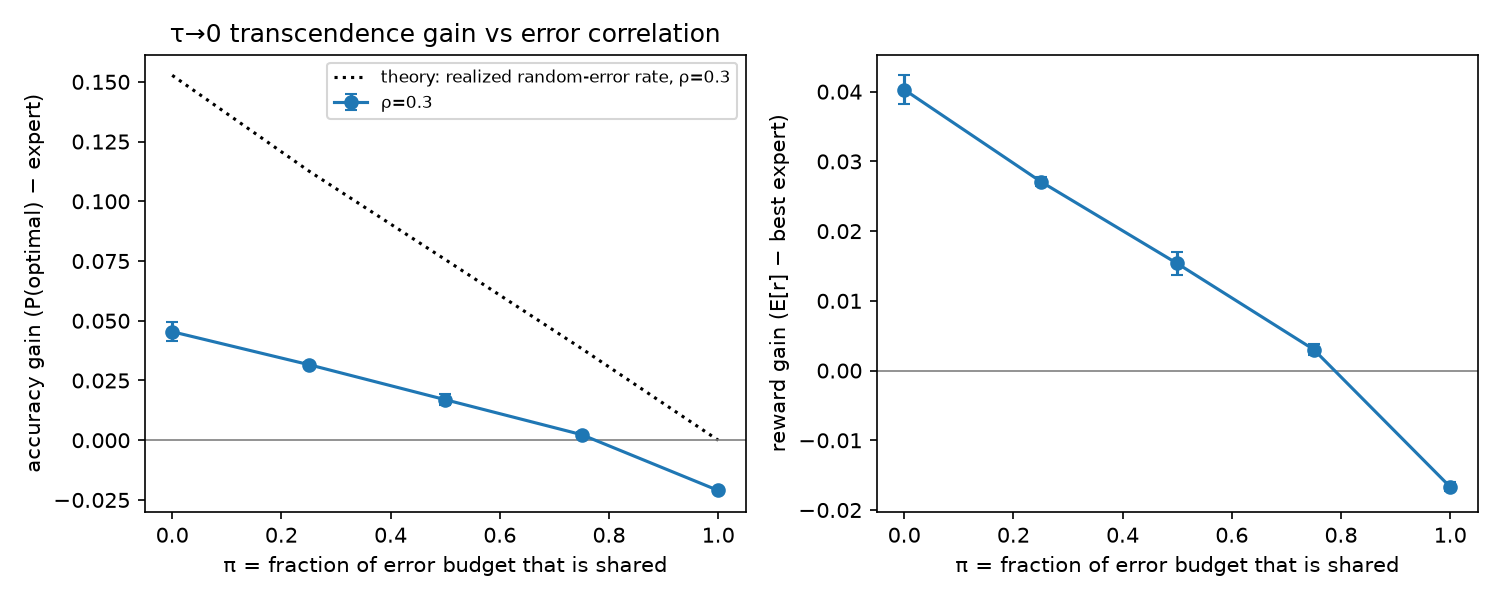
\includegraphics[width=0.49\textwidth]{figs/fig2_gain_vs_pi.png}\hfill
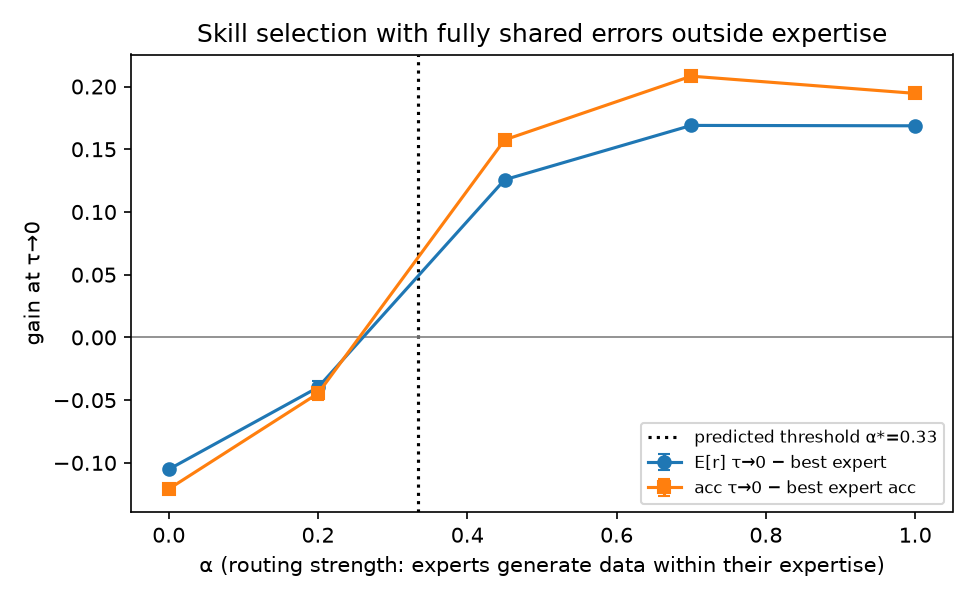
\includegraphics[width=0.49\textwidth]{figs/fig6_selection_alpha.png}
\caption{\textbf{Left:} $\tauz$ gain over the expert as the fraction $\pi$ of shared errors grows at fixed total error rate; dotted line is the theoretical ceiling (realised random-error rate). \textbf{Right:} skill selection with fully shared errors outside expertise; gain over the best expert as a function of routing strength $\alpha$, with the predicted threshold $\alpha^*=1/3$. Three seeds per point; error bars are seed standard deviations and are smaller than the markers.}
\label{fig:validation}
\end{figure}

\begin{table}[t]
\centering\footnotesize
\begin{tabular}{lccccccc}
\toprule
$\pi$ & expert acc & acc $\tau{=}1$ & acc $\tauz$ & theory acc $\tauz$ & $\Er$ gain $\tauz$ & acc on bias states & match $\tauz$ \\
\midrule
0    & 84.5 & 76.2 & 89.1 & 100.0 & $+4.0$ & --   & 71.3 \\
0.25 & 84.6 & 76.4 & 87.8 & 96.2  & $+2.7$ & 40.5 & 62.7 \\
0.5  & 85.7 & 77.9 & 87.4 & 93.5  & $+1.5$ & 42.4 & 63.5 \\
0.75 & 86.6 & 79.4 & 86.8 & 90.5  & $+0.3$ & 39.2 & 62.6 \\
1    & 86.7 & 80.6 & 84.6 & 86.7  & $-1.7$ & 28.6 & 61.4 \\
\bottomrule
\end{tabular}
\caption{Denoising as a function of error correlation $\pi$ (all numbers $\times 100$, three seeds, seed s.d.\ $\le 0.4$). ``Theory acc'' assumes the imitator reproduces every shared error and votes away every random one. ``Match'' is the score against the expert bot.}
\label{tab:pi}
\end{table}

\paragraph{Denoising declines linearly in error correlation.} Table~\ref{tab:pi} and Fig.~\ref{fig:validation} (left). At fixed total error rate the $\tauz$ gain in $\Er$ over the expert is $+0.040,+0.027,+0.015,+0.003,-0.017$ for $\pi=0,0.25,0.5,0.75,1$: monotone, close to linear, and changing sign where Thm.~2 says it must. This is the manipulation the chess paper could not do; the diversity condition is causal, not correlational. The imitator captures about a quarter of the theoretical ceiling (Sec.~\ref{sec:seen} explains where the rest goes).

\begin{table}[t]
\centering\small
\begin{tabular}{lcccccc}
\toprule
$\alpha$ & predicted & best expert acc & mixture acc & acc $\tau{=}1$ & acc $\tauz$ & $\Er$ gain $\tauz$ \\
\midrule
0    & no  & 48.5 & 45.2  & 47.3 & 36.4 & $-10.5$ \\
0.2  & no  & 54.9 & 61.4  & 59.8 & 50.5 & $-4.0$ \\
0.45 & yes & 62.0 & 77.3  & 71.4 & 77.8 & $+12.6$ \\
0.7  & yes & 67.5 & 89.2  & 80.4 & 88.3 & $+16.9$ \\
1    & yes & 78.1 & 100.0 & 94.5 & 97.5 & $+16.9$ \\
\bottomrule
\end{tabular}
\caption{Skill selection with fully shared errors outside expertise ($K=4$, $\alpha^*=1/3$; $\times 100$, three seeds, s.d.\ $\le 0.6$). All three seeds agree with the prediction in every row.}
\label{tab:alpha}
\end{table}

\paragraph{Selection flips at the predicted threshold.} Table~\ref{tab:alpha}, Fig.~\ref{fig:validation} (right). Below $\alpha^*$ low temperature is actively harmful ($-0.105$ at $\alpha=0$): the imitator commits to the shared error. Above it the gain is large and saturates. The sign flips between $0.2$ and $0.45$, as predicted; the transition is smooth rather than a step, because a finite model's argmax follows the mixture margin noisily (accuracy on states with a wrong move available: $0.22,0.60,0.76,0.93$ for $\alpha=0.2,0.45,0.7,1$). Two side observations: at $\tau=1$ the routed mixture already beats the best expert for every $\alpha>0$---selection does not need low temperature, denoising does---and complementary experts (Thm.~4) are transcended by $+0.076$.

\section{The denoising gain lives in recurring states}\label{sec:seen}

\begin{figure}[t]
\centering
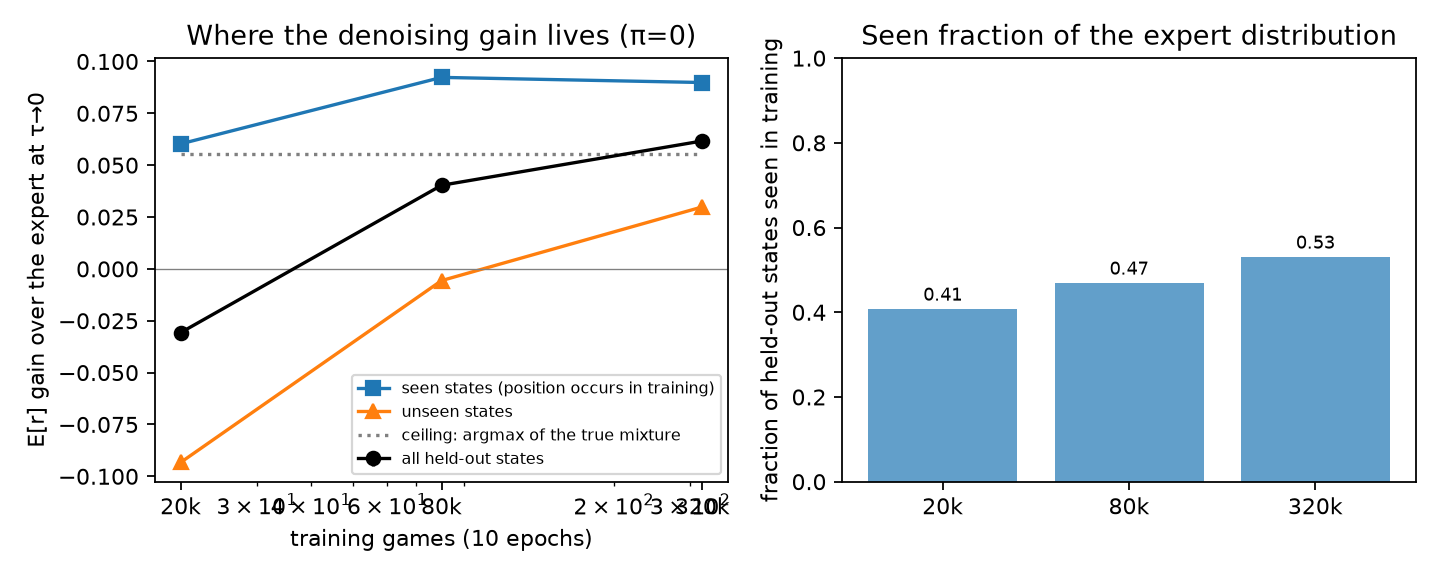
\includegraphics[width=0.95\textwidth]{figs/fig8_datalaw.png}
\caption{Decomposition of the $\tauz$ gain over the expert ($\pi=0$) by whether the held-out position occurs in the training set, as a function of training-set size at a fixed 10 epochs. On seen states the vote reaches the theoretical ceiling from 20k games; on unseen states the imitator is worse than the expert at 20k, equal at 80k and better at 320k. Three seeds at 20k and 80k, one at 320k.}
\label{fig:datalaw}
\end{figure}

Thm.~2 is a statement about a per-state vote. A per-state vote needs per-state votes. Tagging every held-out position as seen or unseen in training splits the $\pi=0$ gain cleanly (Fig.~\ref{fig:datalaw}):

\begin{center}\small
\begin{tabular}{lcccccc}
\toprule
training games & total gain & seen states & unseen states & seen fraction & ceiling (all) & own-play score \\
\midrule
20k  & $-0.031$ & $+0.060$ & $-0.093$ & 0.41 & $+0.055$ & 0.36 \\
80k  & $+0.040$ & $+0.092$ & $-0.006$ & 0.47 & $+0.055$ & 0.72 \\
320k & $+0.062$ & $+0.090$ & $+0.030$ & 0.53 & $+0.055$ & 0.80 \\
\bottomrule
\end{tabular}
\end{center}

On seen states the imitator reaches, and slightly exceeds, the argmax-of-the-mixture ceiling already at 20k games.\footnote{Exceeding it is possible because the ceiling is a per-\emph{move} plurality: when several optimal moves split the correct mass, a single wrong move can carry more mass than any one of them. The theory's ``majority'' is over moves, not over outcome classes.} On unseen states it is first worse than the expert, then equal, then better: generalization-based denoising exists but needs about four times the data at which vote-based denoising saturates. The total gain is the seen-fraction-weighted sum of the two. This is the quantitative form of ``the imitator captures a quarter of the ceiling'': it captures all of it where it has votes and, at 80k games, none of it elsewhere.

A related decomposition explains a puzzle. The $\pi=1$ imitator does not transcend on the experts' state distribution ($-0.017$) yet wins $59\%$ of head-to-head games against the expert bot---while its per-move $\Er$ on its own trajectories is \emph{below} the expert's counterfactual $\Er$ on those same states ($-0.013$). Per-state expected reward and game outcome are different objects: the timing of errors matters for the latter. The chess paper's rating and the taxonomy's query accuracy therefore measure different things, and neither paper says so.

\section{Shared errors survive iff they are representable}\label{sec:repr}

At $\pi=1$ every error is shared, and Thm.~2 says none can be removed. What we observe depends on the phase of the game. On bias states in the opening (positions seen in training) the imitator's $\tauz$ accuracy is $0.006$: the shared error is reproduced exactly. In the middlegame and endgame, where most positions are new, it rises to $0.41$ and $0.56$. The bias states are defined by a hash of the position; nothing about the position predicts them, so on a new position the imitator has no way to know it is a bias state and does what similar positions do, which is the optimal move.

The \emph{rule} condition is the control. Every expert plays the leftmost legal column on plies divisible by three; this is a simple function of the sequence. The imitator's $\tauz$ accuracy on rule plies is $0.248/0.632/0.728$ in opening/middle/endgame---identical, to three decimals, to the accuracy of the rule itself (how often the leftmost column happens to be optimal)---at every checkpoint from step 200 onwards and in every data and training-length variant we ran. The \emph{blind} control behaves the same way: after training on experts that never open in the centre, the imitator puts probability $10^{-4}$ on the centre at $\tau=1$ and $0$ at $\tauz$. No discovery.

The condition in Thm.~2 is therefore not ``shared across experts'' but ``shared across experts \emph{and} representable by the imitator as a function of the state''. Errors that are correlated across the population but unpredictable from the input are removed by generalization, not by voting. Abreu et al.\ state that correlated errors cannot be denoised; this is the missing qualifier.

\section{Training past the memorisation point removes the gain}\label{sec:regime}

\begin{table}[t]
\centering\small
\begin{tabular}{lcccccc}
\toprule
games & steps & epochs & acc $\tau{=}1$ & acc $\tauz$ & final val loss & best val loss (step) \\
\midrule
80k  & 1{,}600  & 10  & 76.3 & \textbf{89.1} & 1.76 & 1.76 (1600) \\
80k  & 6{,}400  & 42  & 78.6 & 83.7 & 2.73 & 1.74 (2400) \\
80k  & 25{,}600 & 167 & 79.0 & 83.5 & 6.63 & 1.74 (2400) \\
320k & 1{,}600  & 2.6 & 75.8 & 88.8 & 1.76 & 1.76 (1600) \\
320k & 6{,}400  & 10  & 78.9 & \textbf{91.4} & 1.69 & 1.69 (6000) \\
320k & 25{,}600 & 42  & 80.7 & 86.5 & 2.18 & 1.69 (8400) \\
\bottomrule
\end{tabular}
\caption{$\pi=0$, one seed. The expert's accuracy is 84.5. Evaluation is at the final checkpoint.}
\label{tab:regime}
\end{table}

Table~\ref{tab:regime}. With 80k games, training from 10 to 42 epochs lowers $\tauz$ accuracy from $0.891$ to $0.837$---below the expert---while the training loss keeps falling and the validation loss explodes. The model memorises the specific noisy games, including their random errors, and its argmax stops being the vote. Four times the data restores the gain and raises it ($0.914$ at 10 epochs) before the same decline sets in. The $\tau=1$ accuracy never reaches the expert's ($0.845$) in any cell: the imitator's distribution is always flatter than its data, so part of the $\tau=1\to\tauz$ improvement removes the model's own residual entropy rather than the experts' noise. This is the memorisation dynamics of Arpit et al.~\cite{arpit2017} and the reason the effect is invisible in a single pass over $10^9$ games: transcendence by low temperature is a property of the regime in which the learner is still estimating the mixture rather than storing the sample. In the $\pi=1$ condition the same overtraining has the opposite surface symptom---the imitator learns fragments of the hash and stops generalizing the shared error away (endgame bias-state accuracy $0.67\to0.50$)---and in the rule condition it changes nothing on rule plies. One mechanism, three symptoms.

\section{Skill composition across demonstrators with disjoint support}\label{sec:composition}

\begin{figure}[t]
\centering
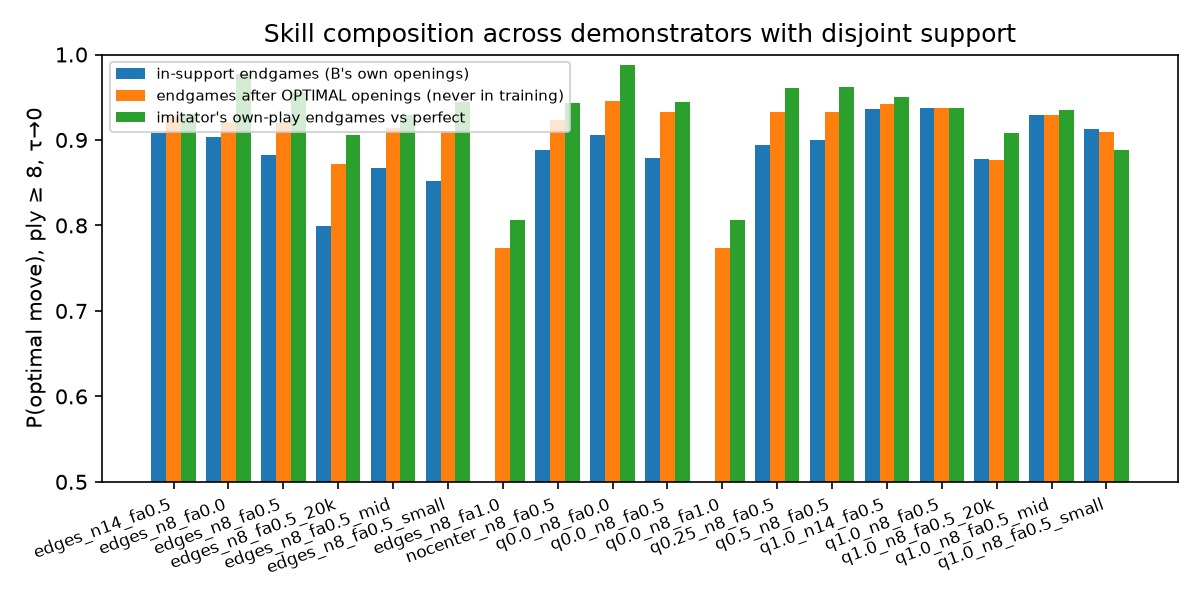
\includegraphics[width=0.98\textwidth]{figs/fig7_composition.png}
\caption{Endgame move accuracy (ply $\ge 8$, $\tauz$) on three state distributions, for every composition condition: positions reached from family B's own openings (in support), positions reached from optimal openings (never in training), and the imitator's own play against a perfect opponent. Bars are means over three seeds. Conditions with $f_A=1$ (family A only) have no in-support endgames.}
\label{fig:composition}
\end{figure}

Zhang et al.\ prove transcendence for complementary experts under the assumption that every expert is defined on the whole state space and note that this cannot hold in practice past the opening. Abreu et al.\ test composition on two-hop facts and obtain weak results ($34\%$ without chain of thought). The question---does an imitator compose the skills of demonstrators whose supports do not overlap?---is one on which informed positions disagree: the taxonomy's two-hop numbers and the stitching failures of return-conditioned imitation~\cite{paster2022,brandfonbrener2022} predict collapse, while compositional generalization in chess transformers~\cite{meszaros2025} predicts transfer. The training signal is silent, not contradictory, on the states in question, so the mixture-argmax theory makes no prediction: the answer is a property of the learner's inductive bias.

\begin{table}[t]
\centering\footnotesize
\resizebox{\textwidth}{!}{%
\begin{tabular}{llcccc}
\toprule
& & \multicolumn{2}{c}{endgame acc after \emph{optimal} openings} & \multicolumn{2}{c}{own play vs.\ perfect} \\
condition ($N{=}8$ unless noted) & family B opening & mid / late & $\Delta$ vs control & acc open/mid/late & score \\
\midrule
control & optimal ($q{=}1$)        & 0.950 / 0.926 & --              & 0.999 / 0.958 / 0.918 & 0.402 \\
        & random ($q{=}0$)         & 0.940 / 0.924 & $-0.010/-0.002$ & 0.995 / 0.946 / 0.943 & 0.371 \\
        & nocenter                 & 0.926 / 0.920 & $-0.024/-0.006$ & 0.997 / 0.936 / 0.951 & 0.349 \\
        & edges                    & 0.925 / 0.916 & $-0.025/-0.010$ & 0.999 / 0.953 / 0.958 & 0.342 \\
\midrule
A only ($f_A{=}1$)  & --  (no endgames at all) & 0.868 / 0.680 & $-0.082/-0.246$ & 0.997 / 0.835 / 0.779 & 0.193 \\
B only ($f_A{=}0$)  & edges                    & 0.919 / 0.924 & $-0.031/-0.002$ & 0.873 / 0.983 / 0.971 & \textbf{0.000} \\
\midrule
$N{=}14$            & edges (control 0.961/0.923) & 0.945 / 0.910 & $-0.016/-0.013$ & 0.999 / 0.971 / 0.891 & 0.407 \\
0.1M-param model    & edges (control 0.927/0.891) & 0.918 / 0.904 & $-0.009/+0.013$ & 0.988 / 0.946 / 0.944 & 0.236 \\
0.8M-param model    & edges (control 0.941/0.917) & 0.924 / 0.905 & $-0.017/-0.012$ & 0.995 / 0.924 / 0.933 & 0.282 \\
20k games           & edges (control 0.904/0.850) & 0.890 / 0.855 & $-0.014/+0.005$ & 0.996 / 0.904 / 0.907 & 0.204 \\
\bottomrule
\end{tabular}}
\caption{Composition across demonstrators with disjoint support. Family A: optimal opening, transcript truncated at ply $N$. Family B: opening of the stated kind, optimal endgame. ``After optimal openings'' evaluates the imitator's logits on endgame positions reached from optimal openings, which appear in no transcript. Own play: 300 games against a solver-perfect opponent, alternating colours; a perfect first player wins Connect~4, so the maximum score is $0.5$. Three seeds per row, s.d.\ $\le 0.005$ on accuracies.}
\label{tab:composition}
\end{table}

Table~\ref{tab:composition} and Fig.~\ref{fig:composition} give the answer in this domain: \textbf{it transfers, with a small graded penalty.} Endgame skill demonstrated exclusively on positions reached from edge-column openings is applied to positions reached from optimal openings at $0.925$ accuracy against $0.950$ for the control that saw them. The penalty grows with the severity of the shift (random $<$ nocenter $<$ edges) and is essentially unchanged by truncating later ($N=14$), by a $60\times$ smaller model, or by $4\times$ less data. There is no cliff anywhere.

The controls make the composition claim precise. Family B alone transfers just as well ($0.919$): family A's transcripts contribute nothing to the endgame. What A contributes is the opening. B alone plays edge-style openings (accuracy $0.873$) and \emph{loses every game} against the perfect opponent; A alone has never seen a move past ply 8 and collapses in the endgame ($0.680$); the imitator trained on both plays near-perfect openings ($0.999$) and near-perfect endgames ($0.953/0.958$) and wins about $70\%$ of its first-player games against a perfect opponent---a full game that no member of either demonstrator population can play. A side observation: family A alone, having never seen a ply beyond 8, still plays the middlegame at $0.868$; it extrapolates the structure of optimal openings well past its support before collapsing late.

We read this as a clean, quantitative confirmation of the optimist position for a fully observed Markov game: the endgame policy the imitator learns is a local function of the board, not a lookup over the demonstrator's trajectories, even though the imitator sees only move sequences and must build that board representation itself from edge-only histories. It is the empirical content the taxonomy's \emph{skill generalization} mode lacked. It is not a surprise to those who expected it; it is a measurement where before there was a disagreement.

\section{Discussion}

\paragraph{One estimator, several symptoms.} Every deviation from the two theories that we measured is a property of the learned argmax as an estimator of the true one: it is exact where a position recurs (Sec.~\ref{sec:seen}), it has a bias toward functions of the state (Sec.~\ref{sec:repr}), it has variance around the mixture margin (the smooth selection threshold), and it overfits to the sample (Sec.~\ref{sec:regime}). None of these is a new phenomenon in machine learning. Their value here is that they are measured against an exact theoretical object, in the exact places the theory leaves open.

\paragraph{What this says about the chess result.} The 1000-to-1500 gain of~\cite{zhang2024transcendence} is measured on the model's own play against an engine. Our decomposition suggests reading it as three components: a vote on recurring positions (the opening and early middlegame), generalization on new positions that only helps at very large data---which they had---and the removal of the model's own residual entropy, which is not transcendence over the experts at all. Their single pass over $10^9$ games kept them out of the memorisation regime that destroys the first component.

\paragraph{Limitations.} Connect~4 is small, fully observed and exactly solved; the reward is an outcome class, not a fine-grained value. Our experts are synthetic and their errors are by construction either independent or perfectly shared; human errors are neither. The composition result concerns a Markov policy in a game where board features are local; it does not speak to composing declarative knowledge, where the two-hop results of~\cite{abreu2025taxonomy} remain the relevant evidence. Most scaling cells have one seed and evaluate the final checkpoint rather than the best one. And the domain makes the optimist's prediction on composition the plausible one; a domain where the pessimist's prediction were plausible would be a stronger test.

\paragraph{Related work.} Beyond the two papers we build on, the closest empirical work is Krestnikov~\cite{krestnikov2026}, who shows in synthetic arithmetic that coherent minority-false answer systems win over the truth while random errors do not; our $\pi$ and representability results are the sequential-decision counterpart, with the distinction that our shared errors are exceptions to a rule supported by the rest of the data rather than competing rule systems. Compositional generalization of chess transformers to unseen positions is documented by M\'esz\'aros et al.~\cite{meszaros2025}; stitching failures of trajectory imitation by Paster et al.~\cite{paster2022} and Brandfonbrener et al.~\cite{brandfonbrener2022}. The memorisation dynamics we observe are those of Arpit et al.~\cite{arpit2017}. The reversal curse~\cite{berglund2023} and the knowledge-manipulation results of Allen-Zhu and Li~\cite{allenzhu2023} bound what one should expect from symmetric-relation repair, which is why we did not attempt it.

\paragraph{Reproducibility.} All code, expert generators, datasets, trained models and the chronological log of the experiments are released at \url{https://github.com/marianocrosetti/c4-transcendence}\sloppy{}. The full set of runs cost under \$20 of GPU time.

\subsubsection*{Acknowledgements}
Experiments, analysis and drafting were carried out with Claude (Anthropic) acting as an autonomous research assistant; all design decisions, interpretations and errors are the author's.

\begin{thebibliography}{9}
\small
\bibitem{zhang2024transcendence} E.~Zhang, V.~Zhu, N.~Saphra, A.~Kleiman, B.~L.~Edelman, M.~Tambe, S.~M.~Kakade, E.~Malach. Transcendence: Generative models can outperform the experts that train them. \emph{NeurIPS}, 2024. arXiv:2406.11741.
\bibitem{abreu2025taxonomy} N.~Abreu, E.~Zhang, E.~Malach, N.~Saphra. A taxonomy of transcendence. \emph{COLM}, 2025. arXiv:2508.17669.
\bibitem{allis1988} V.~Allis. A knowledge-based approach of Connect-Four. Master's thesis, Vrije Universiteit Amsterdam, 1988.
\bibitem{pons2019} P.~Pons. Connect 4 game solver. \url{http://connect4.gamesolver.org}, 2019.
\bibitem{arpit2017} D.~Arpit et al. A closer look at memorization in deep networks. \emph{ICML}, 2017.
\bibitem{meszaros2025} A.~M\'esz\'aros, P.~Reizinger, F.~Husz\'ar. Out-of-distribution tests reveal compositionality in chess transformers. arXiv:2510.20783, 2025.
\bibitem{paster2022} K.~Paster, S.~McIlraith, J.~Ba. You can't count on luck: Why decision transformers and RvS fail in stochastic environments. \emph{NeurIPS}, 2022.
\bibitem{brandfonbrener2022} D.~Brandfonbrener, A.~Bietti, J.~Buckman, R.~Laroche, J.~Bruna. When does return-conditioned supervised learning work for offline reinforcement learning? \emph{NeurIPS}, 2022.
\bibitem{krestnikov2026} A.~Krestnikov. Truth as a compression artifact in language model training. arXiv:2603.11749, 2026.
\bibitem{berglund2023} L.~Berglund et al. The reversal curse: LLMs trained on ``A is B'' fail to learn ``B is A''. arXiv:2309.12288, 2023.
\bibitem{allenzhu2023} Z.~Allen-Zhu, Y.~Li. Physics of language models: Part 3.2, knowledge manipulation. arXiv:2309.14402, 2023.
\end{thebibliography}

\appendix
\section{Additional details}

\paragraph{Realised error rates.} With nominal $\rho=0.3$ the realised per-state error rate of the iid experts is $0.15$, because an error is only possible in the $52\%$ of visited positions where some legal move has a worse outcome class. The theory rows of Table~\ref{tab:pi} use realised shared and random error rates measured on the test set.

\paragraph{Selection margin.} Accuracy on states where a wrong move is available, at $\tauz$: $0.132, 0.223, 0.597, 0.759, 0.931$ for $\alpha=0,0.2,0.45,0.7,1$. The mixture margin between the optimal and the shared wrong move is $-0.5,-0.2,+0.175,+0.55,+1$.

\paragraph{Representability, all cells.} Rule plies accuracy of the imitator equals $0.248/0.632/0.728$ (opening/middle/late) in every one of: three seeds at 80k games; 80k and 320k games at 1{,}600, 6{,}400 and 25{,}600 steps; and every 200-step checkpoint of the 80k run. The rule itself (leftmost legal column) is optimal with exactly those frequencies. Hash-bias accuracy ($\pi=1$, 80k, 10 epochs) is $0.006/0.412/0.561$; with 320k games and 10 epochs $0.000/0.378/0.666$; with 320k games and 42 epochs $0.000/0.233/0.503$.

\paragraph{Own-play decomposition for $\pi=1$.} On the experts' distribution: seen states $60\%$ of positions ($99.9\%$ of opening, $46\%$ of middlegame, $1.5\%$ of endgame); gain $-0.004$ on seen, $-0.036$ on unseen. On the imitator's own trajectories against the expert bot (300 games, score $0.587$): gain $-0.003$ on seen, $-0.032$ on unseen, by phase $-0.001/-0.010/-0.078$.

\paragraph{Compute.} Data generation is CPU-bound in the solver ($\approx 2$\,ms per position); an 80k-game dataset takes 20 minutes on 8 cores. Training 1{,}600 steps takes 30 minutes on an Apple M4 (MPS) and 1.7 minutes on an RTX~4090. In total: 13 base conditions $\times$ 3 seeds, a 12-cell scaling study, 16 composition conditions $\times$ 3 seeds, and 8 decompositions.

\end{document}
